\documentclass[10pt]{beamer}

\usetheme[progressbar=frametitle]{metropolis}
\usepackage{appendixnumberbeamer}
\usepackage[style=authoryear, backend=bibtex8, natbib=true, maxcitenames=2]{biblatex}

\usepackage{amsmath}
\usepackage{xcolor}

\usepackage{graphicx}
\usepackage{import}

\usepackage{booktabs}
\usepackage[scale=2]{ccicons}

\usepackage[utf8]{inputenc}

\usepackage{pgfplots}
\usepgfplotslibrary{dateplot}

\usepackage{xspace}
\newcommand{\themename}{\textbf{\textsc{metropolis}}\xspace}

\title{Opgaver til kapitel 19}
\subtitle{Handel}
% \date{\today}
\date{\today}
\author{Kristian Olesen Larsen}
\institute{Department of Economics, University of Copenhagen}

\begin{document}
\setbeamercolor{background canvas}{bg=white}
\maketitle






% Syntax: \colorboxed[<color model>]{<color specification>}{<math formula>}
\newcommand*{\colorboxed}{}
\def\colorboxed#1#{%
  \colorboxedAux{#1}%
}
\newcommand*{\colorboxedAux}[3]{%
  % #1: optional argument for color model
  % #2: color specification
  % #3: formula
  \begingroup
    \colorlet{cb@saved}{.}%
    \color#1{#2}%
    \boxed{%
      \color{cb@saved}%
      #3%
    }%
  \endgroup
}


% ------------------------------------------------------------------------------
% ------ FRAME -----------------------------------------------------------------
% ------------------------------------------------------------------------------
\section{Opgave 1}

\begin{frame}{a) Transformationskurven}
  \begin{figure}
  \centering
      \includegraphics<1>[width=0.8\textwidth]{img/clean}
      \includegraphics<2>[width=0.8\textwidth]{img/step1}
      \includegraphics<3>[width=0.8\textwidth]{img/step2}
\end{figure}

\only<1>{Transformationskurven knytter de mulige produktionsniveauer af forskellige varer sammen.}

\only<2>{
Alle er ansat i brødindustrien $\rightarrow$ dem der er dygtigst til at bygge biler skifter branche $\rightarrow$ Bilproduktionen stiger meget, mens brødproduktionen kun falder lidt.
}

\only<3>{
Nu arbejder næsten alle i bilindustrien $\rightarrow$ de dygtigste bagere forlader branchen.
}
\end{frame}


% ------------------------------------------------------------------------------
% ------ FRAME -----------------------------------------------------------------
% ------------------------------------------------------------------------------
\begin{frame}{b) Influenza blandt de ansatte}
Landet rammes af en voldsom influenzaepidemi, hvad sker der?

\begin{itemize}
\item Influenza $\approx$ reduceret arbejdsstyrke
\item Der er både færre arbejdere til at producere brød og biler
\item Hele kurven rykker nedad
\only<2> {
\item (Hvor meget rykker den ned?)
}
\end{itemize}

\end{frame}

\begin{frame}{c) Ny brødblandingsmaskine}

    \begin{figure}
    \centering
        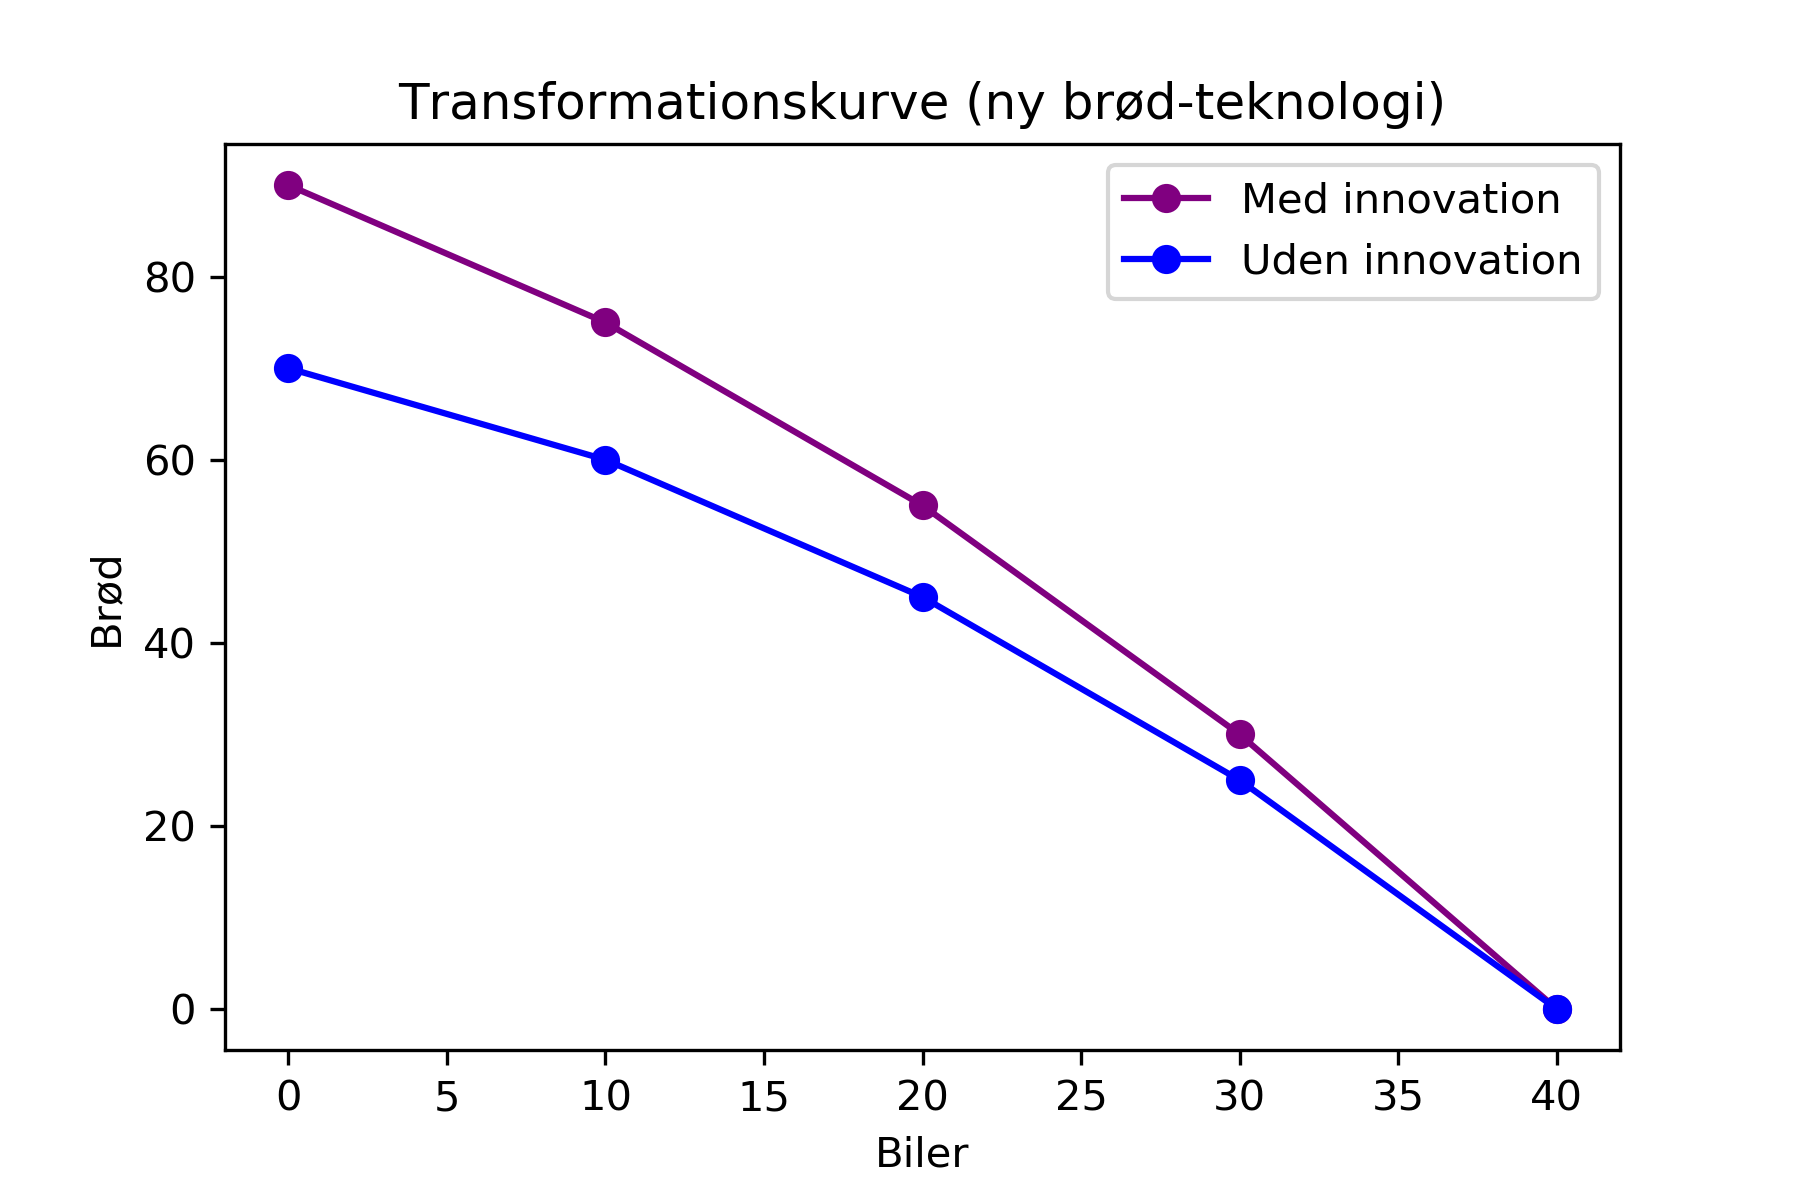
\includegraphics[width=0.8\textwidth]{img/innov}
  \end{figure}

Maskinen øger produktionen hos hver enkelt bager $\rightarrow$ mange ansatte giver stor samlet produktionsstigning.

\end{frame}


\begin{frame}{d) Arbejdsløshed}

    \begin{figure}
    \centering
        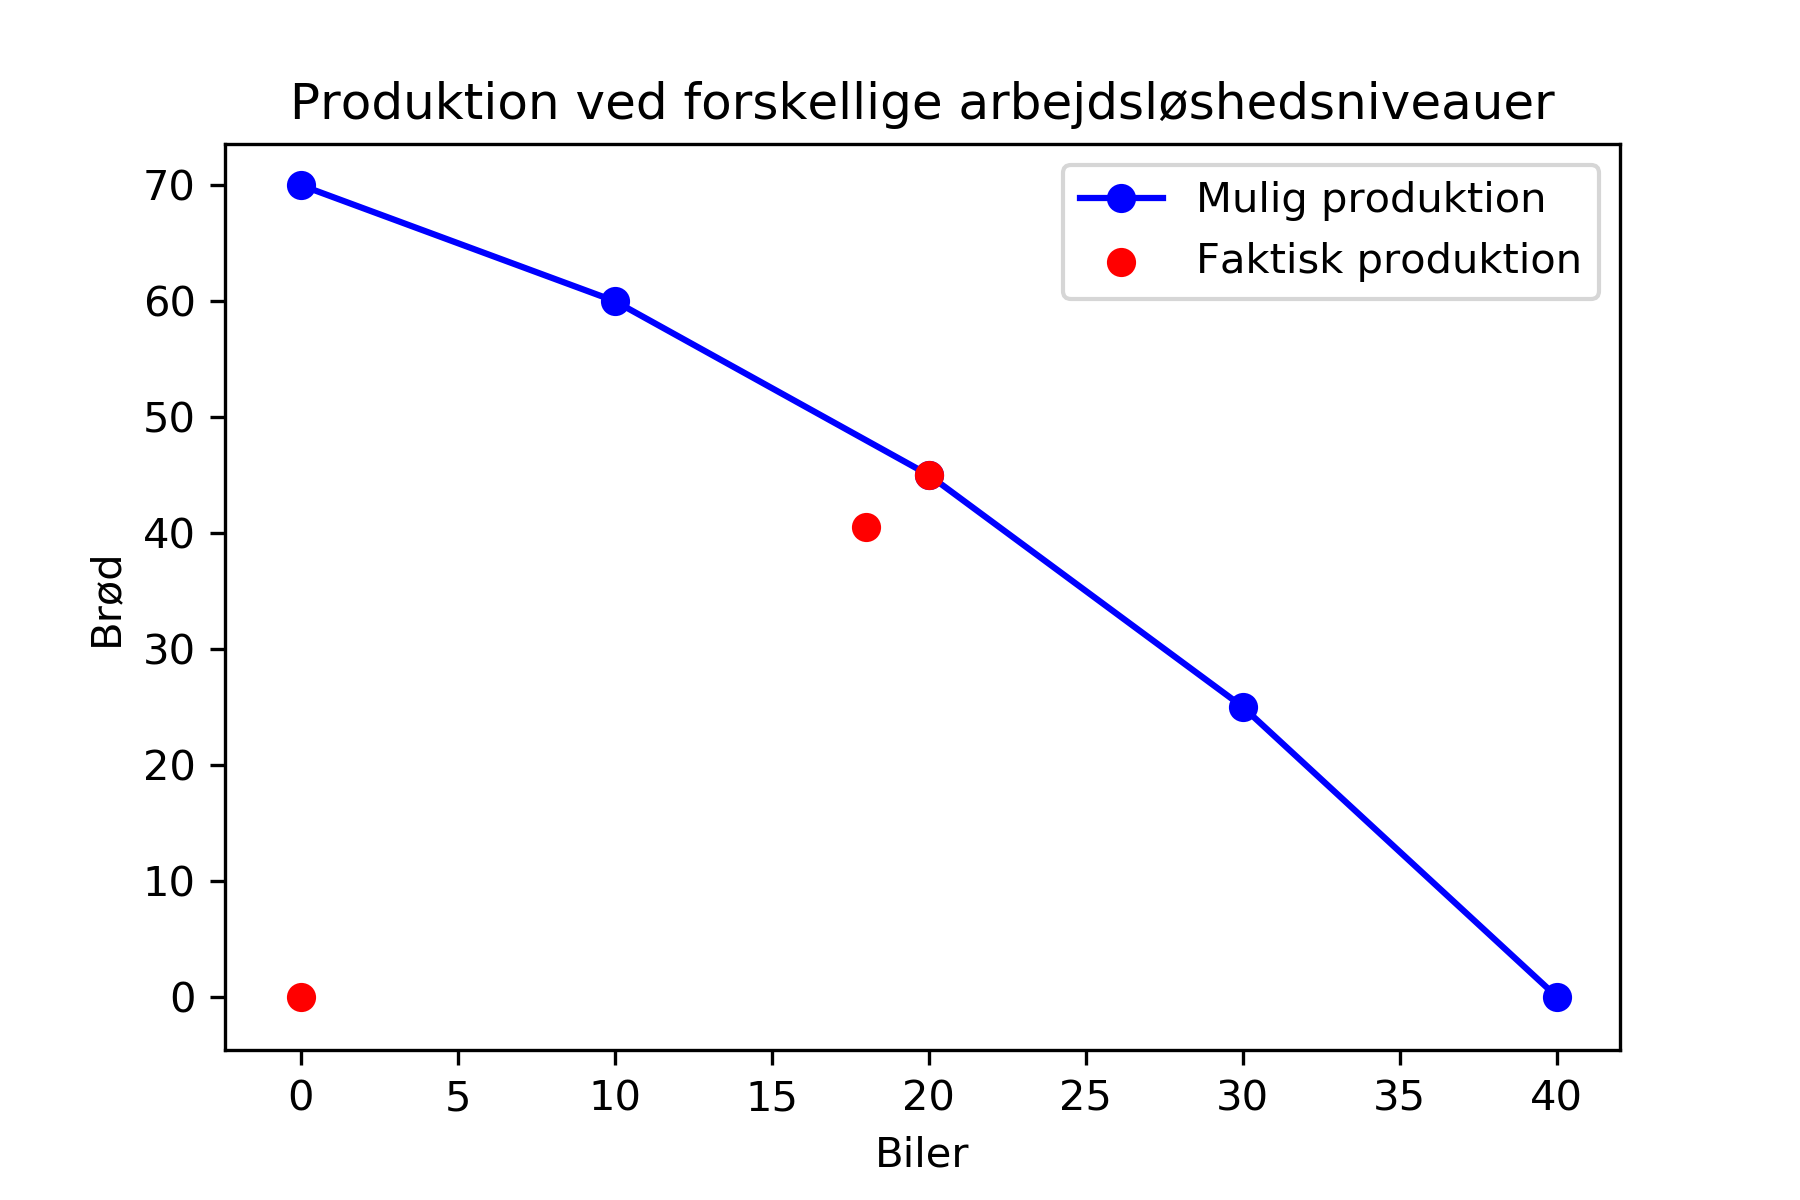
\includegraphics[width=0.8\textwidth]{img/unemp}
  \end{figure}

  \begin{itemize}
      \item[0\%] Fuld udnyttelse af potentialet i økonomien
      \item[10\%] Produktionen ligger lidt under transformationskurven
      \item[100\%] Ingen arbejder $\rightarrow$ ingen produktion $(x_1,x_2) = (0,0)$
  \end{itemize}

\end{frame}


\section{Opgave 2}

\begin{frame}
Søren og Ole er biologer der er taget til Alaska. Søren kan maksimalt producere 10kg fisk eller 6kg rensdyr. Ole kan fange 5kg fisk eller 8kg rensdyr.

Kan handel stille begge bedre? Hvordan? 
\end{frame}

\begin{frame}{a) Søren og Ole i vildmarken}
Søren: 10kg fisk eller 6kg rensdyr, Ole: 5kg fisk eller 8kg rensdyr.

Uden handel: $(fisk, \ rensdyr) = (6kg, \ 5kg)$
Maksimal produktion: $(fisk, \ rensdyr) = (10kg, \ 8kg)$

\only<2,3>{
\begin{itemize}
\item Kan handel stille både Søren og Ole bedre?
  \begin{itemize}
    \item Ja! Søren laver 10kg fisk og bytter for Oles 8kg rensdyr.
  \end{itemize}
\item Kan handel øge den samlede produktion?
  \begin{itemize}
    \item Ja!
  \end{itemize}
\end{itemize}
}

\only<3>{Hvorfor er 10kg fisk og 8kg rensdyr den maksimale produktion?}

\end{frame}


\section{Opgave 3}

\begin{frame}
Peter kan producere 4 liter vand eller 2 skiver brød, mens Hans kan producere enten 2 liter vand eller 1,5 skiver rugbrød.

Kan handel stille begge bedre?
\end{frame}

\begin{frame}{a) Transformationskurver}

    \begin{figure}
    \centering
        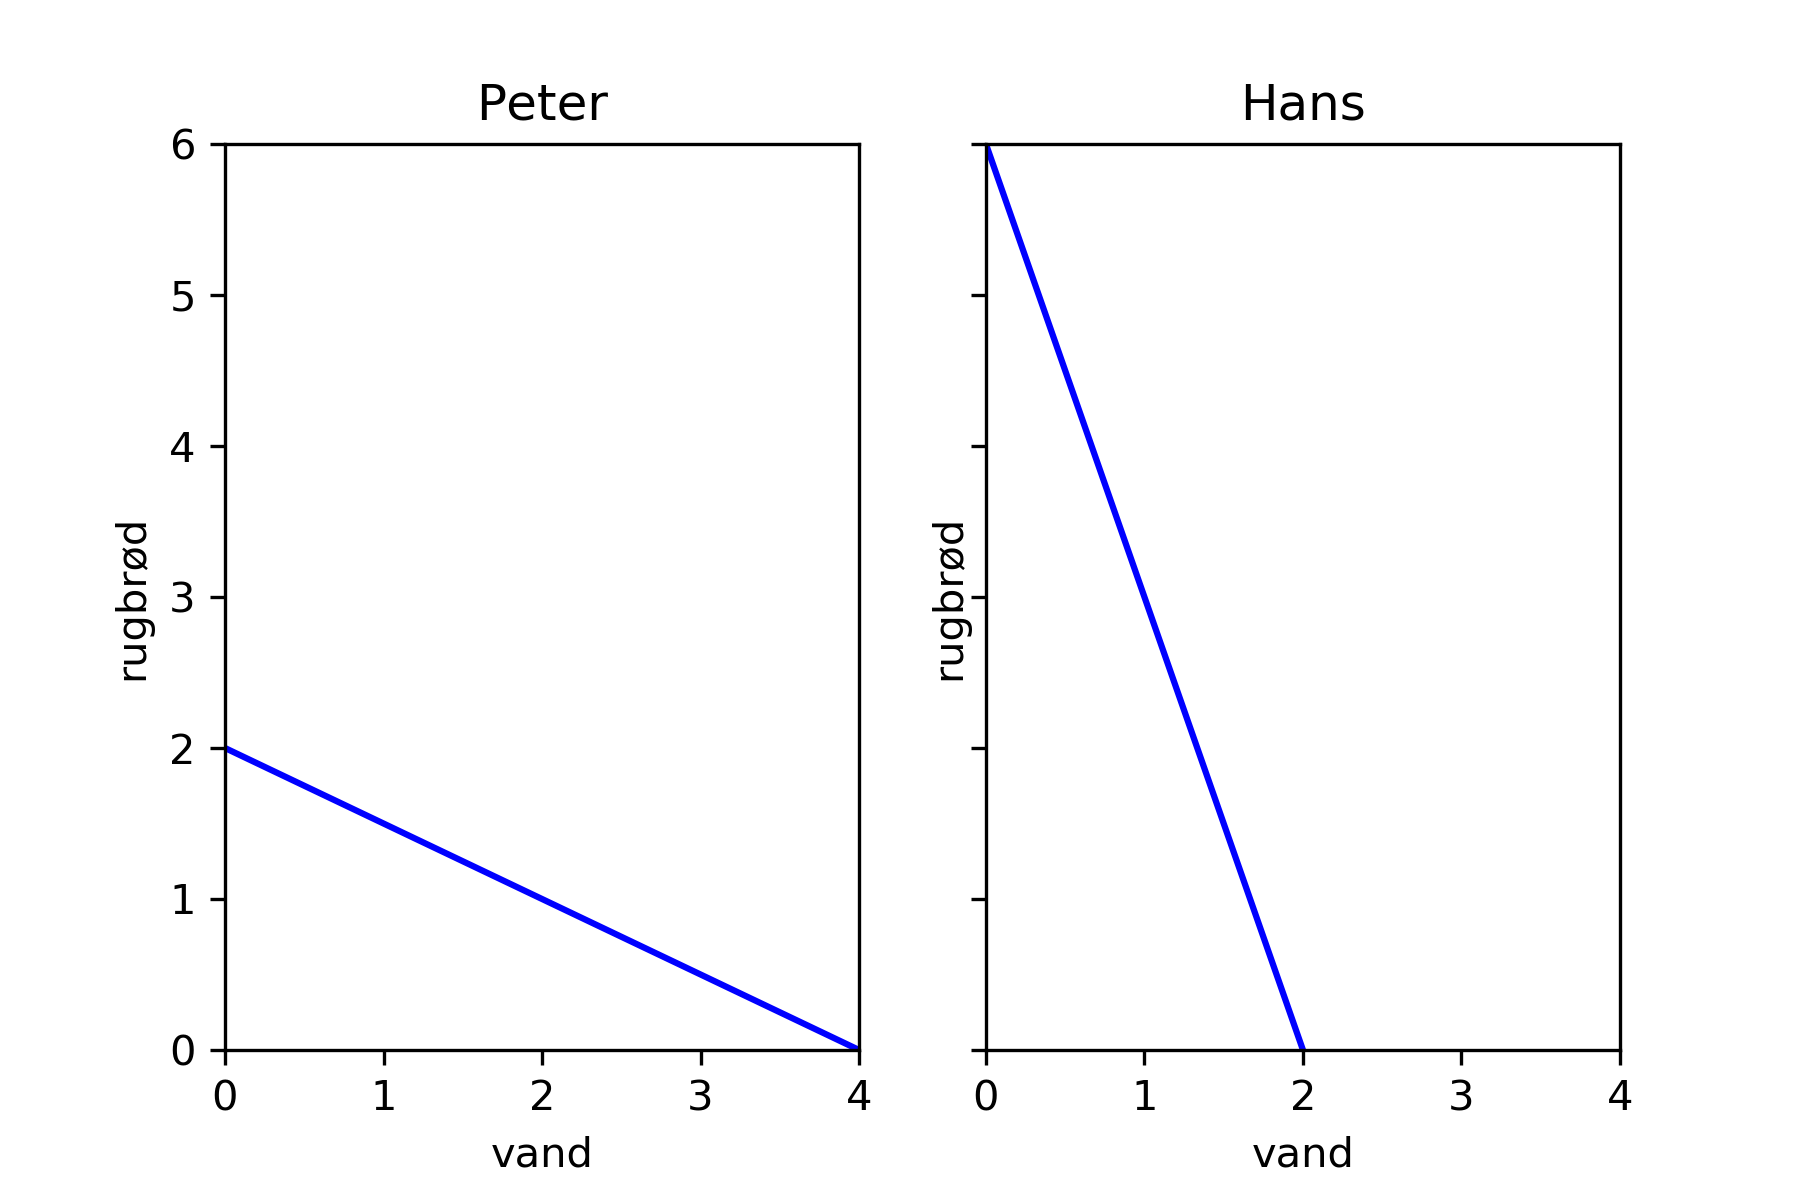
\includegraphics[width=0.8\textwidth]{img/comp1}
  \end{figure}

\end{frame}


\begin{frame}{b) Absolutte og komparative fordele}


  \begin{itemize}
    \item[Peter:] $R = 2 - \only<2>{\colorboxed{red}} {\frac{2}{4} \only<2>{}} v \qquad \Leftrightarrow \qquad v = \colorboxed{blue}{4}-2R$
    \item[Hans:] $R = \colorboxed{blue}{6} - \frac{6}{2}v \qquad \Leftrightarrow \qquad v = 2 - \only<2>{\colorboxed{red}}{\frac{1}{3} \only<2>{}}R$
    \item[]
    \item[Total?] $R_P + R_H = 2 - \frac{2}{4}v +  6 - \frac{6}{2}v = 8 - (\frac{1}{2} + 3)v$
  \end{itemize}

\begin{itemize}
  \item \textcolor{blue}{Absolute fordele:}
  \begin{itemize}
    \item \textit{Absolutte fordele $=$ mest produktion pr. tidsenhed}
    \item Peter har absolut fordel i at producere vand, fordi han kan producere 4 liter pr. dag, Hans kan kun producere 2 liter pr. dag.
  \end{itemize}
\only<2>{\item \textcolor{red}{Komparative fordele:}
  \begin{itemize}
    \item \textit{Komparative fordele $=$ laveste alternativomkostninger ved produktion}
    \item Peter har også komparativ fordel i at producere vand. Han skal kun opgive $\frac{1}{2}$ kg rugbrød for at lave 1 liter vand. Hans skal opgive 3 liter vand, for at få 1 kg rugbrød.
  \end{itemize}
}
\end{itemize}

\end{frame}

\begin{frame}{c) Kan handel stille Peter og Hans bedre?}

    \begin{figure}
    \centering
        \includegraphics<1>[width=0.8\textwidth]{img/komp2}
        \includegraphics<2>[width=0.8\textwidth]{img/komp2_solve}
  \end{figure}

\only<2,3>{Godt nok må begge opgive noget, men de får stadig begge to samlet set et bedre outcome.

Kan de gøre det endnu bedre ved at ændre produktion?}

\end{frame}


\begin{frame}{ d) Har Hans incitament for at dele ligeligt med Peter?}

  \begin{itemize}
    \item Hans har måske lyst til selskab i huset?
    \item Diskuter ...
  \end{itemize}

\end{frame}


\section{Opgave 4}

\begin{frame}
Smith og Ricardo siger at lande skal specialisere sig i at producere varer de er relativt bedst til. Hvilke varer forventer vi at importere/eksportere fra Danmark til Kina? Hvad viser handelsmønstrene os?
\end{frame}


\begin{frame}{Hvilke varer har Danmark en komparativ fordel i at producere?}

Hvordan svarer man på sådan et spørgsmål?
\begin{itemize}
  \item[1)] Hvilke varer eksporterer Danmark egentligt til Kina? $\rightarrow$ det må være dem vi har en komparativ fordel i!
  \item[2)] Hvilke varer har lave alternativomkostninger at producere i Danmark? $\rightarrow$ kan vi gætte det?
\end{itemize}

\end{frame}


\section{Opgave 5}

\begin{frame}
Anders og Helle lever i en lukket økonomi, hvor der kun forbruges fisk og kartofler. Anders kan producere 2kg fisk eller 1kg kartofler, mens Helle kan producere 1kg fisk eller 2kg kartofler. Både Helle og Anders vil kun forbruge de to goder i forholdet 1:1.

Kan de begge stilles bedre ved at handle?
\end{frame}

\begin{frame}{a) Produktionsmulighedsområdet}
\begin{itemize}
  \item Ugentlig produktion (hvis de udelukkende producerer 1 vare)
  \begin{itemize}
    \item Anders: $(F,K)_A = 6\cdot (2,1) = (12,6)$
    \item Helle: $(F,K)_H = 6 \cdot (1,2) = (6, 12)$
  \end{itemize}
\end{itemize}
\begin{figure}
\centering
    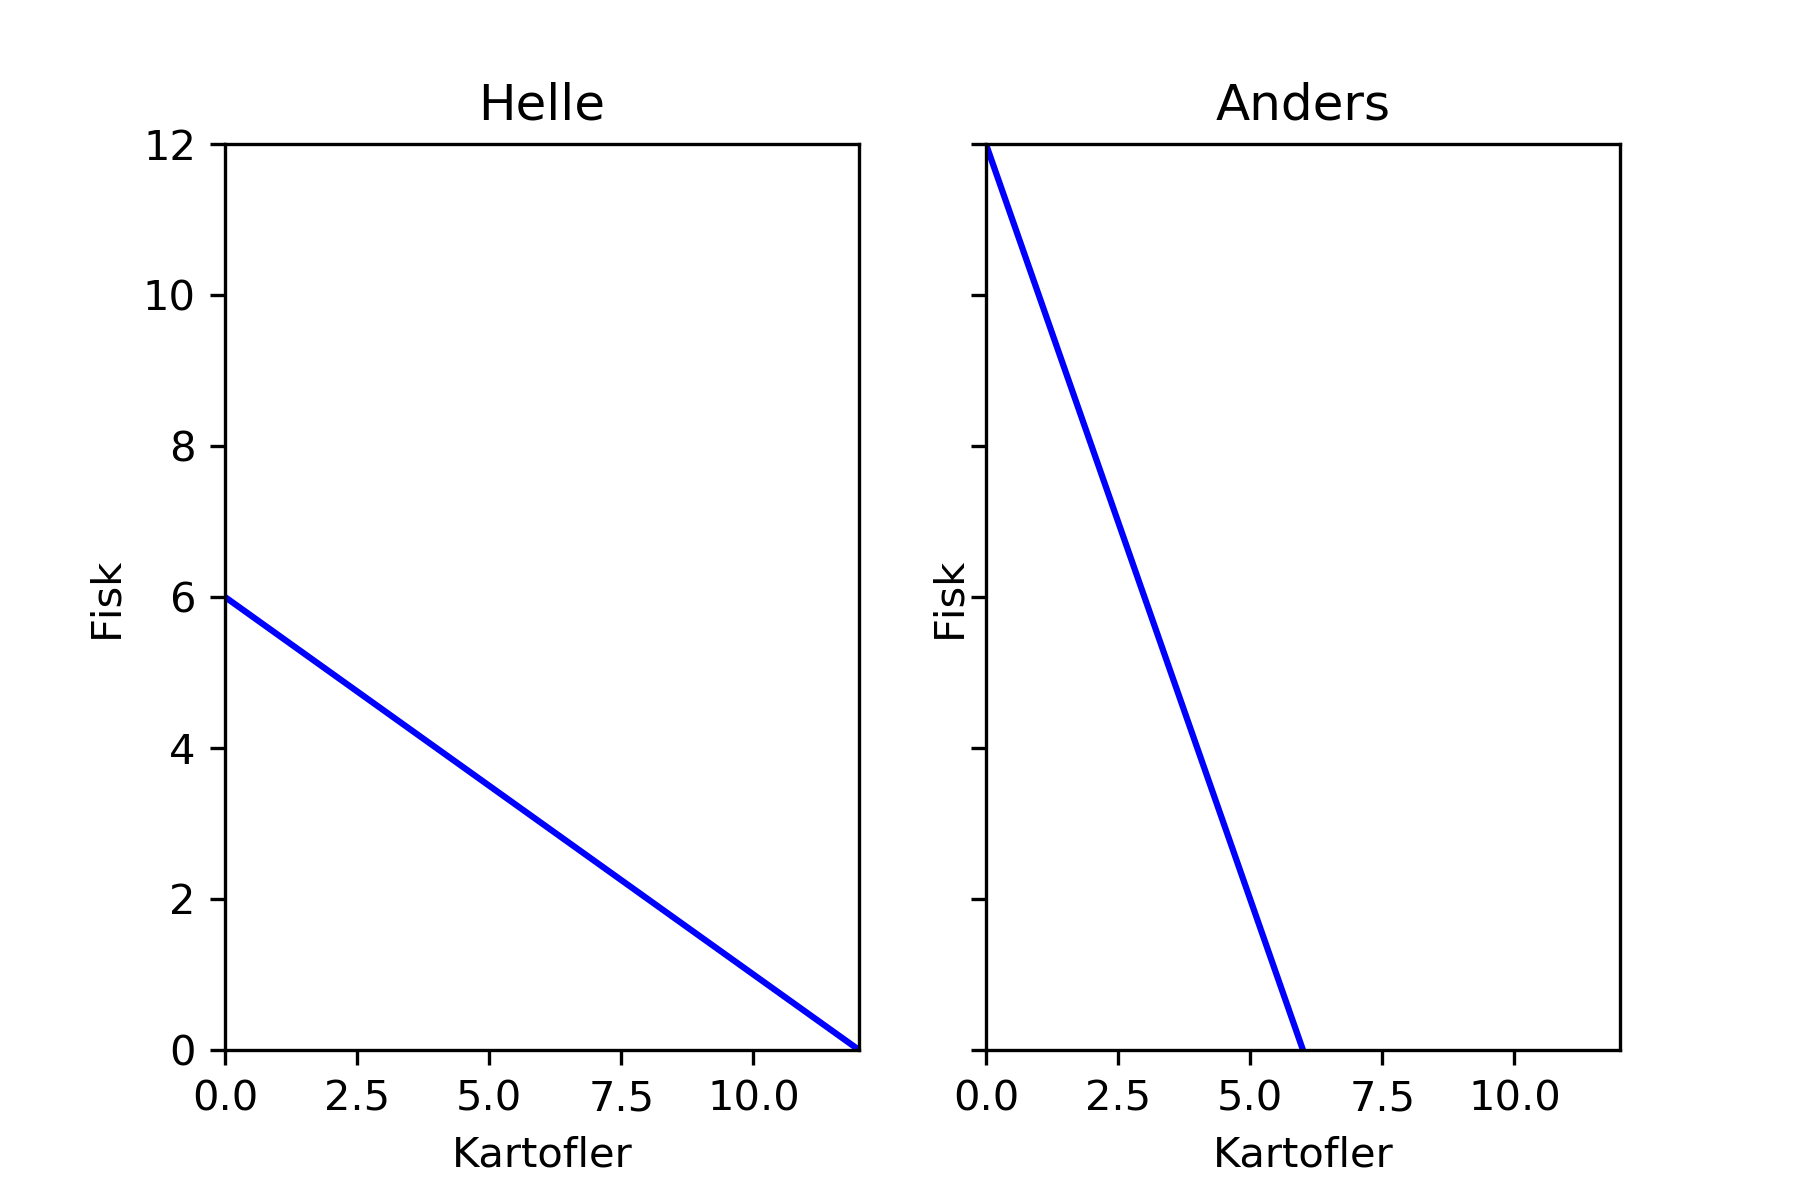
\includegraphics[width=0.6\textwidth]{img/comp2}
\end{figure}
Hvad er ligningerne for de to linjer?
\only<2>{\begin{itemize}
  \item Anders: $F_A(K_A) = 12 - 2K_A$
  \item Helle: $F_H(K_H) = 6 - \frac{1}{2}K_H$
\end{itemize}}
\end{frame}


\begin{frame}{b) Forbrug uden handel}
Husk at de begge kun vil forbruge lige dele fisk og kartofler, så for dem begge gælder at $F=K$.

\textbf{Anders:}
\begin{align*}
  F_A &= 12-2K_A \\
  & = 12 - 2F_A \\
  F^*_A &= 4
\end{align*}
Indsæt $F_A = 4$ i den oprindelige ligning
\begin{align*}
  4 &= 12 -2K_H \\
  K^*_H &= 4
\end{align*}
\textbf{Helle:}

Vi kunne gøre som for Anders, men fordi $F_H(K) = F_A^{-1}(K)$ og $F_A^*=K_A^*$ er løsningen $(F_H^*, F_K^*) = (4,4)$.
\end{frame}


\begin{frame}{c) Produktionsmulighedsområde og alternativomkostninger?}

\begin{itemize}
  \item \textbf{Hvad er sammenhængen mellem produktionsmulighedsområdet og alternativomkostningerne?}
  \begin{itemize}
    \item Hældningen på området er en alternativomkostning - \textit{"Hvis Helle øger produktionen af kartofler med 1kg, må hun sænke produktionen af fisk med $\frac{1}{2}$kg".}
  \end{itemize}
  \item \textbf{Hvem har de komparative fordele?}
  \begin{itemize}
    \item Kartofler: Helle. Hun skal kun sænke produktionen af fisk med 1/2 kg for at producere 1kg kartofler ekstra.
    \item Fisk: Anders. Hvorfor?
  \end{itemize}
\end{itemize}

\end{frame}


\begin{frame}{d) Påvirker handel situationen?}

Antag fuld specialisering - så producerer Anders 12kg fisk, og Helle 12kg kartofler. De vil kun forbruge i forholdet 1:1, så de kan bytte 6kg fisk for 6kg kartofler og forbruge $(F,K)=(6,6)$.

\end{frame}

\begin{frame}{d) Påvirker handel situationen?}
\begin{figure}
\centering
    \includegraphics<1>[width=0.9\textwidth]{img/comp2_analysis}
    \includegraphics<2>[width=0.9\textwidth]{img/comp2_analysis_arrow}
\end{figure}

\end{frame}


\begin{frame}{e) Ændring i Helles produktion}
Læg mærke til at ændringen øger helles produktion af både fisk og kartofler forholdsmæssigt lige meget. Derfor er der stadig komparative fordele.

De absolute fordele Anders havde i produktion af fisk er dog forsvundet.
\end{frame}


\section{Opgave 6}

\begin{frame}{a) Gør-det-selv arbejde}
Nej - det giver ikke mening at højt specialiseret arbejdskraft laver gør-det-selv arbejde. Det har håndværkere komparative fordele i.
\end{frame}


\section{Opgave 7}

\begin{frame}{a) Kornpriser}

Hvis $p^{\textrm{verden}}>p^*$, er det så til gavn for de indenlandske producenter at åbne for handel med verden?


\only<2>{Nej (se Claus' slides for gennemgang)}
\end{frame}

\section{Opgave 8}


\begin{frame}{a) Håndværksmarkedet}

Hvis $p^{\textrm{verden}}<p^*$, er det så til gavn for de indenlandske producenter at åbne for handel med verden?

Eller med andre ord: hvad betyder det for danske håndværkere og forbrugere at blive udsat for konkurrence fra østeuropæiske håndværkere?

\only<2>{Det svarer til opgave 7, men nu er $p^{\textrm{verden}}<p^*$}
\end{frame}




\end{document}
